\chapter{Introduction}


%==================================================================================================
\section{Introduction}

%--------------------------------------------------------------------------------------------------
\subsection{Motivation}
I have encountered a problem that was insipration for this work during my research in field
of mobile robotics. While my initial focus was directed more towards emergent behaviour in 
robotics and a self organizing systems I have encountered a issue with localization in marine 
robotics. With high cost of internet connection for robots operating far away from land it 
is important to be able to calculate precise position without updating data from internet.
One of issuse when working with satellite navigation system is requirement for clock bias
correction, to keep error drift to minimum readouts for both local and satellite clock must
be corrected by predicted bias. In this work I focused on prediction of errors in satellite
clocks as unlike in case of local clock those can be later reused by other people.


%--------------------------------------------------------------------------------------------------
\subsection{History of robotics}

%--------------------------------------------------------------------------------------------------
\subsection{Acknoweledgements}

%==================================================================================================
\section{Robot navigation}

%--------------------------------------------------------------------------------------------------
\subsection{Basic concepts}
Unlike a robotic manipulators for which there is always a single joint fixed to a specific
location in external reference frame mobile robot must be equipped with a way to localize
themselves in environment.
\begin{figure}[hb]
	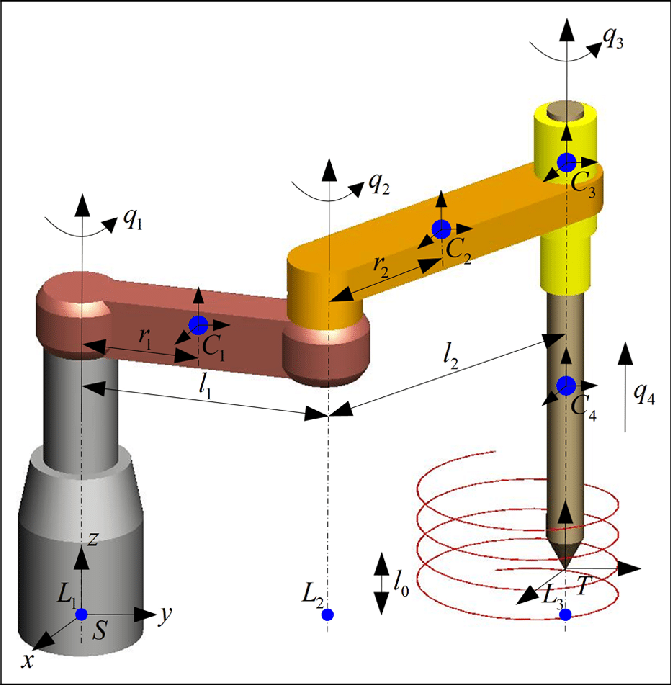
\includegraphics[width=0.5\textwidth]{res/robot_arm_reference}
	\caption{Kinematic chain of robotic manipulatr}
	\label{fig:robot_arm_reference}
\end{figure}


%--------------------------------------------------------------------------------------------------
\subsection{Reference versus dead reckoning}

%--------------------------------------------------------------------------------------------------
\subsection{Beacon based navigation}
All Global Satellite Navigation systems (GNSS) are variant of beacon-based localization
systems\cite{Blewitt1997}. Such systems require information about the beacon position
and distance between the localized object and beacons.
With that information, it is possible to calculate the position of an object in the same reference
frame as that of beacons.
Both of those tasks are much more difficult in GNSS due to the nature of the beacons.
Unlike in the case of stationary beacons, GNSS satellites move at high speed so
their position must be calculated based on satellite ephemerides.
Another problem is how to measure distance with use of reasonably priced reciever while 
maintaining high level of precision.
There are three possible approaches to a beacon based localisation:
\begin{itemize}
	\item Time of Arrival (ToA),
	\item Angle of Arrival (AoA),
	\item Received Signal Strength (RSS).
\end{itemize}
AoA detects at which angle a beacon signal arrives and reqires a specialised receiver capable 
of such measurements. This type of localization requires a complex reciever and do not provide 
a satisfactionary precision when dealing with such remote objects as a satellites.
While RSS can work with a very simple reciever its precision is low for signals that, like
the GPS signal, are designed with low power loss over large distances.
This leaves ToA as only valid solution, when measuring distance by ToA 
three properties of a signal should be known:
\begin{itemize}
	\item $t_o$ - time of origination,
	\item $t_a$ - time of arrival,
	\item $v$ - velocity.
\end{itemize}
In case of GNSS signal is an electromagnetic wave therefore its speed is equal
to a speed of light $c$. Time of arrival is recorded when
data frame wavefront reaches the receiver, this means that receiver time is used.
Signal generation time is recorded on satellite according to its local clock and
included in the data frame. Thanks to that distance can be calculated by simple
equation:
\begin{equation}
	d=c(t_a-t_o).
\end{equation}
However $t_a$ and $t_o$ are using different reference frame so for comparison
to be possible they must be transformed into a common reference frame.
This is referred to as a synchronization of the clocks and is very important as
a desynchronization on the level of a single nanosecond results in about 30 cm of
positioning error\cite{Enge2011}.

%==================================================================================================
\section{Global navigation satellite systems}

%--------------------------------------------------------------------------------------------------
\subsection{GPS}

%--------------------------------------------------------------------------------------------------
\subsection{GLONASS}

%--------------------------------------------------------------------------------------------------
\subsection{Galileo}

%--------------------------------------------------------------------------------------------------
\subsection{Others}




